
%(BEGIN_QUESTION)
% Copyright 2006, Tony R. Kuphaldt, released under the Creative Commons Attribution License (v 1.0)
% This means you may do almost anything with this work of mine, so long as you give me proper credit

Explain what will happen (and why!) in this pneumatic proportional controller if the bias spring breaks in half:

$$\includegraphics[width=15.5cm]{i01496x01.eps}$$

Furthermore, explain what effect this fault would have on the process being controlled by this pneumatic controller.  In other words, what will happen to the value of the process variable as a result of the bias spring breaking, assuming no adjustments are made to the controller by any person?

\vfil 

\underbar{file i01496}
\eject
%(END_QUESTION)





%(BEGIN_ANSWER)

This is a graded question -- no answers or hints given!

%(END_ANSWER)





%(BEGIN_NOTES)

The first step in any analysis of a pneumatic feedback mechanism is to determine whether the mechanism is {\it force-balance} or {\it motion-balance}.  Only then may we accurately assess the consequences of various changes made to the mechanism.

\vskip 10pt

If the bias spring breaks, the controller output will decrease because that spring will no longer impart a downward force on the beam near the output bellows.  With less downward force applied to the left-hand side of the beam, the output bellows will not have to ``fight back'' as hard to balance the beam, resulting in less output pressure than before the spring breakage.

Since this cessation of downward force (by the spring) constitutes a {\it subtraction} of force in the system, we know the effect will be a ``zero shift'' in the mechanism rather than a ``span shift'' (which would require a multiplication or division of force).  Thus, we know the broken spring must affect the {\it bias} of the controller and not the {\it gain}.

\vskip 10pt

As for the effect of this fault on the process variable being controlled, we need to first determine the direction of this controller's action.  It is a reverse-action controller, which means an increasing PV results in a decreasing output.  If this is indeed the appropriate action for the process being controlled, it means the process itself must be ``direct-acting'' (i.e. an increase in control valve opening results in an increase in PV).  The ``action'' of a process must always be opposite that of its loop controller in order for the control feedback to be negative (stable).

Thus, knowing this process responds directly to changes in output from the controller, we may conclude that the PV will likewise decrease as a result of the output decreasing due to the spring break.

A helpful problem-solving strategy here is to imagine a real process example that would function well with a reverse-acting controller, and then see what would happen to that process if its controller suddenly suffered a decrease in bias.  For example, we might imagine the process to be a water-level control, where an air-to-open control valve allows fresh water to enter the vessel to increase its level.  This process clearly needs a reverse-acting controller (more water level = shut valve).  If the valve in this process happens to suddenly close off a bit due to the spring's breakage, it will result in a (slight) decrease in water level.

%INDEX% Control, proportional: pneumatic force-balance controller

%(END_NOTES)


